\section*{Reviewer 1}
\vspace{-2mm}
\paragraph{R1.1} We have extended the introduction to discuss the advantages and disadvantages of PSG and why it is not applicable to our
problem. See also R4.1. Thanks for the comments.

\paragraph{R1.2} Embarrassed not to have introduced and provided sufficient details on our pilot study. This information is now given in Section 3.1.
\vspace{-2mm}
\paragraph{R1.3} We take 12-28 samples every minute to detect respiratory events. This is based on the observation that an adult typically
breathes around 15 times per minute. We found that this setting is effective for our problem. This is now clarified in Section 2.1.2.

\paragraph{R1.4} The 10 volunteers involved in the training data process (pilot study) for determining the algorithm parameters are different from the 15 users recruited in our
evaluation. The data were collected while they were sleeping. This is clarified in Section 2.1 in the revised manuscript.

\paragraph{R1.5} Our HMM model is trained using our training dataset. This is now clarified in Section 2.4. See also R1.4.
\vspace{-2mm}
\paragraph{R1.6} To evaluate our approach, we have randomly picked at least 3 sets of data from each of our 15 testing users.
The current submission is not evaluated on the full dataset (which contains videos of over 1,000 hours) due to the time constraint (as we
need to watch each video to mark out sleep events). That said, we are able to demonstrate the usefulness of our approach on a relatively
small but representative set of data. We are currently working to extend our evaluation to the entire dataset. The results will be ready
for and included in the camera ready paper.

\paragraph{R1.7} ``invasive" is indeed a poorly chosen word for describing Fibit. We have reworded.
\vspace{-2mm}
\paragraph{R1.8} The signals shown in Fig.5 are indeed from a single subject. This is clarified in the revised version.
\vspace{-2mm}
\paragraph{R1.9} Our work uses respiratory events to distinguish if a hand is put on the chest or the shoulder. Although the shoulder is
next to the chest, we observed that it is less likely to be affected by respiration, i.e., there is fewer changes in the speedometer
readings when the hand is put on the shoulder over the chest. Hence, we can distinguish the hand position by measuring the respiratory
events. This is now clarified in Section 2.1.2.

%\textcolor{blue}{According to our observations and tests, when the hand was placed on the shoulder, the wrist was affected
%little by the respiratory event. This is because the way the hand is placed makes the wrist to have a certain space from the chest. Fig.
%\ref{Bodyhand} shows the trajectory data of the hands moving from the side of the body to the chest and shoulder respectively. We can see
%that the obvious respiratory events cannot be observed when the hand is put on the shoulder.}

%\begin{figure}[!t]
%	\centering
%	\subfigure[]{\label{BodytoChest}
%		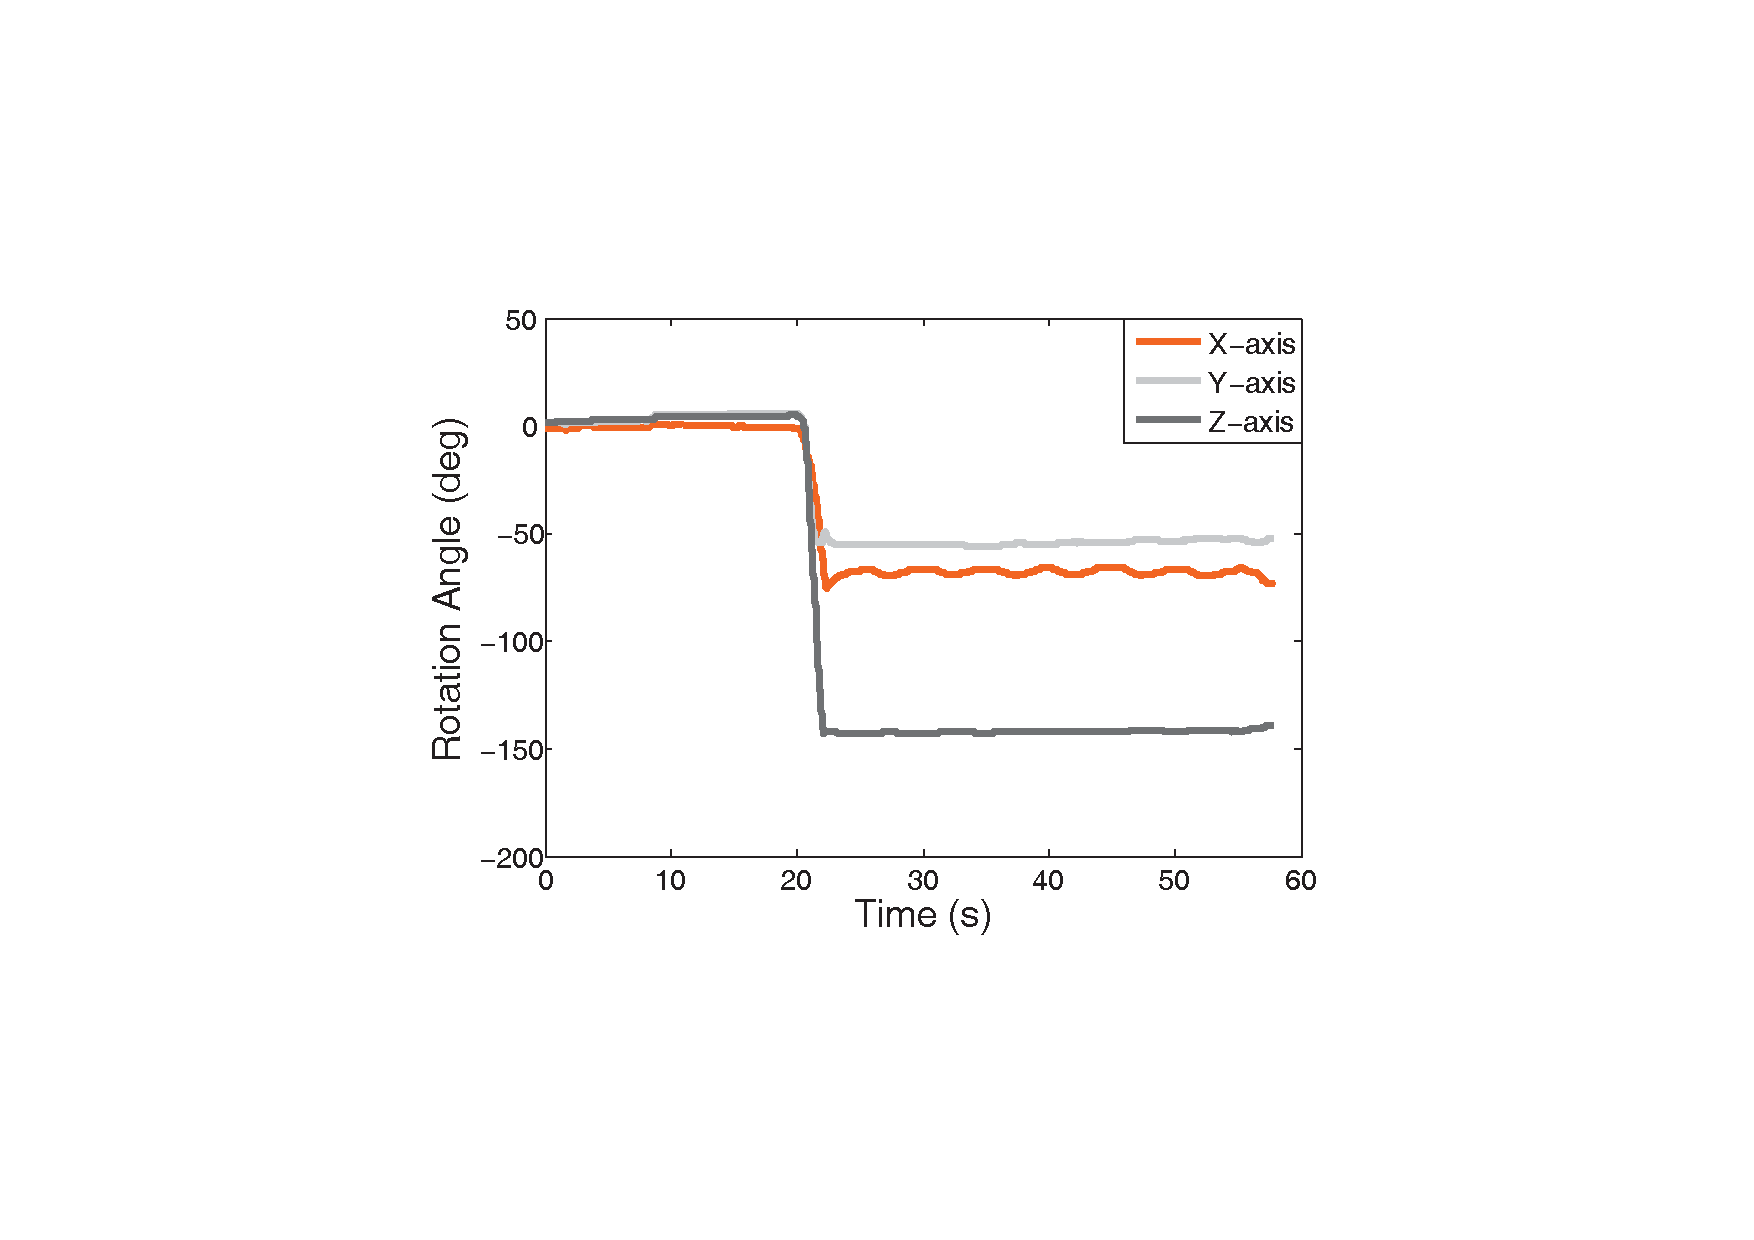
\includegraphics[width=0.32\linewidth]{Figures/BodytoChest.pdf}}
%	%  \hfill
%	\subfigure[]{\label{BodytoShoulder}
%		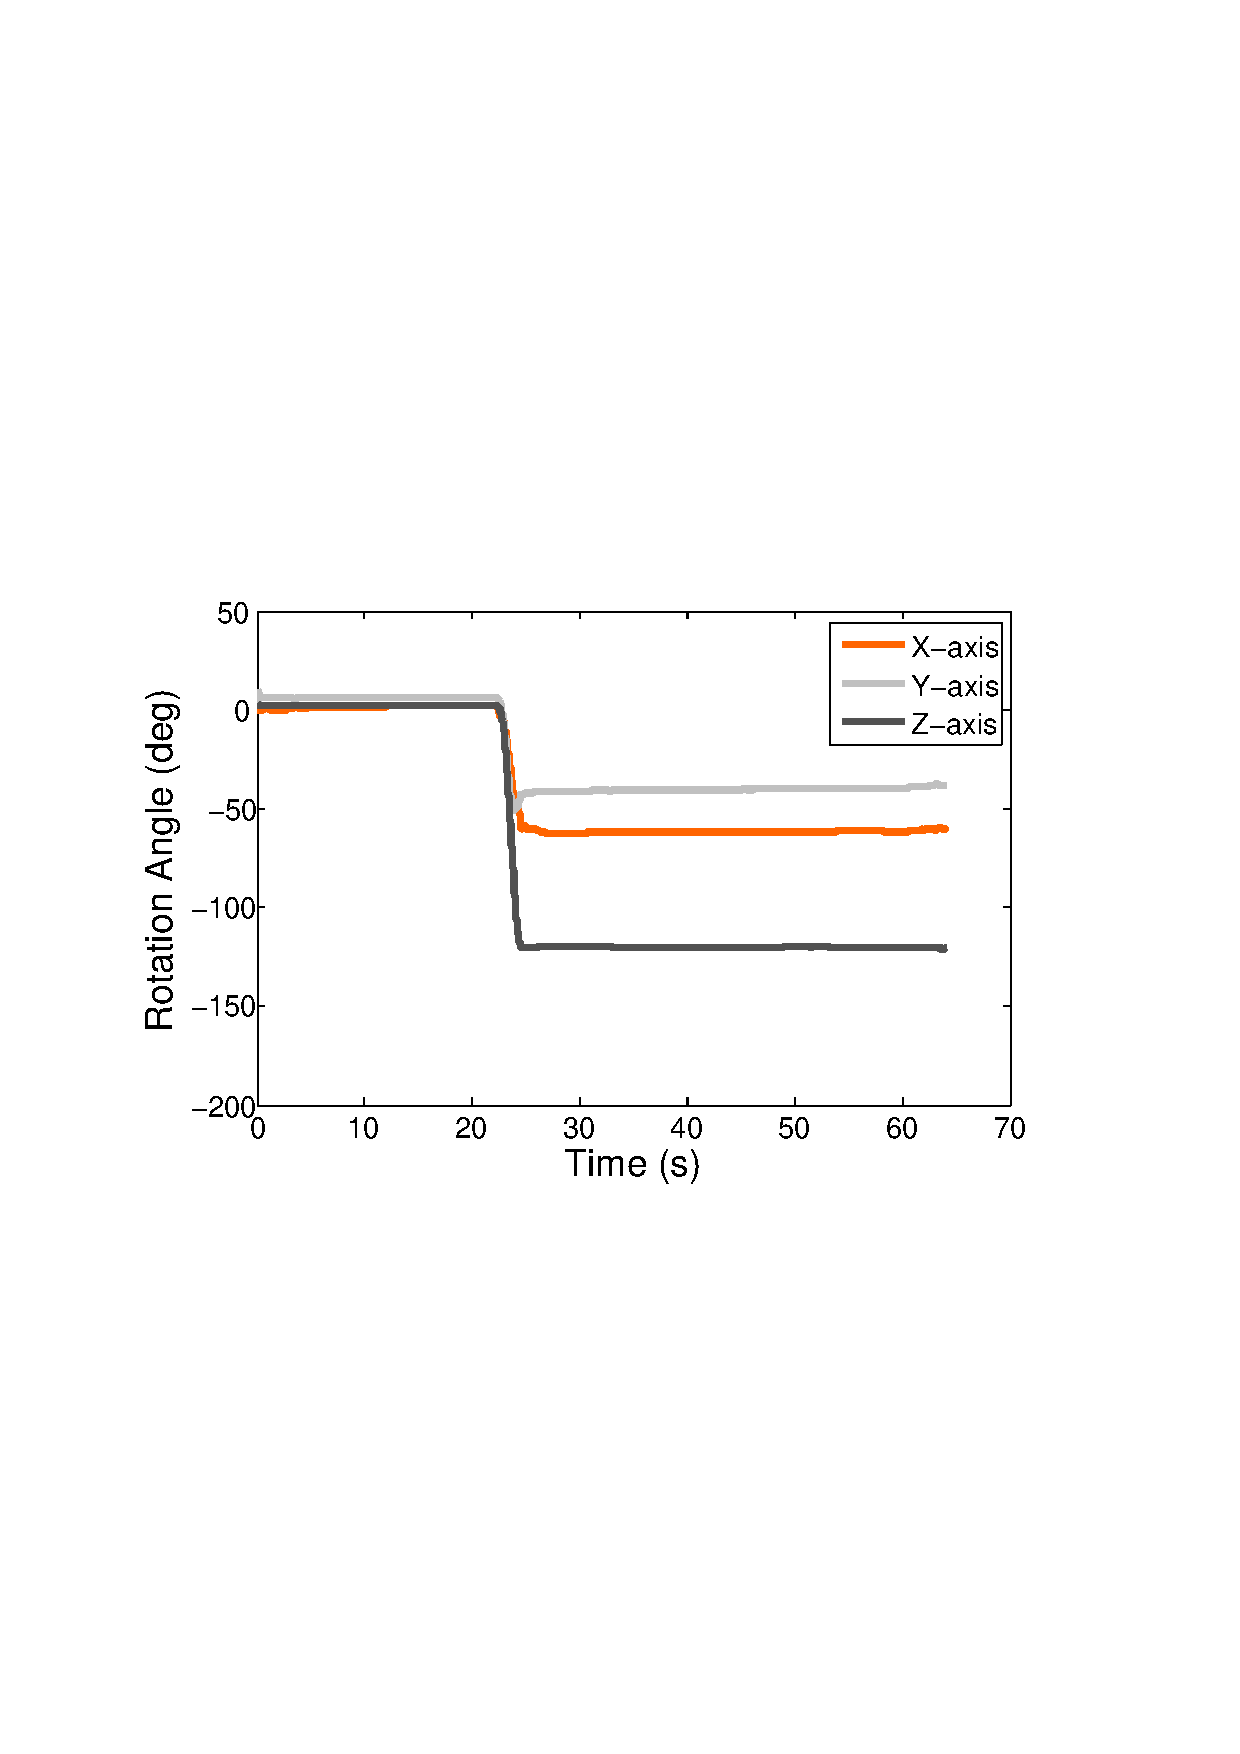
\includegraphics[width=0.34\linewidth]{Figures/BodytoShoulder.pdf}}
%	\caption{The characteristics of hand movement from the position beside the body  to (a)  the chest, and (b) the shoulder.}\label{Bodyhand}
%\end{figure}


\paragraph{R1.10} Good catch, the sentence should be instead read as ``A body rollover event is recorded when the posture changes are detected between
two time points". We have now amended the texts in the revised version.

\paragraph{R1.11} We have given the parameters for the moving average filter in Section 2.1.4 in the revised version. Thanks.
\vspace{-2mm}
\paragraph{R1.12} The acceleration threshold was determined from training data. This is now clarified in Section 2.1.4. See also
R1.4. \vspace{-2mm}
\paragraph{R1.13} Our algorithm does consider a situation where the wrist turns so that the back of the hand become downward. This is now clarified in Section 2.3.
\vspace{-2mm}
\paragraph{R1.14} The reviewer is right that there is no standard definition for sleep stages. We have provided our definitions of the various stages per reviewer suggestions in Section 2.4.

\paragraph{R1.15} We have extended Section 5 to discuss how our approach can be extended to a multi-sleeper scenario.
\vspace{-2mm}
\paragraph{R1.16} The ground truth of micro-body movements are obtained through (a) watching videos and (b) using the phone accelerometer data. We use the accelerometer data because visions of subtle body movements sometimes can be blocked due to the filming camera angles or surrounding objects (e.g., quilt). This is clarified in Section 4.1.4.

\paragraph{R1.17} We have provided a more detailed analysis and discussion for Table 9 in Section 4.2.4.
\vspace{-2mm}
\paragraph{R1.18} Discussing on the frequency of unusual arm positions is a great point. This is now included in Section 5.
\vspace{-2mm}
\paragraph{R1.19} We have make all the minor corrections and fixed the presentation issues. Many thanks for the feedback.
